%REPORT TEMPLATE
%AUTHOR: RUI QU  
%EMAIL: RQU@KTH.SE 

%----------------------------------------------------------------------------------------
%	PACKAGES AND DOCUMENT CONFIGURATIONS
%----------------------------------------------------------------------------------------

\documentclass{article}

%---Basic---
\usepackage{natbib} % Required to change bibliography style to APA
\usepackage{amsmath} % Required for some math elements 
\setlength\parindent{0pt} % Removes all indentation from paragraphs
\usepackage{listings}%Insert code
\usepackage{times} % Uncomment to use the Times New Roman font

%---Table---
\usepackage{multirow}%Table
\usepackage{booktabs}%Table Triple-lines
\usepackage{siunitx} % Provides the \SI{}{} and \si{} command for typesetting SI units

%---Figure---
\usepackage{graphicx} % Required for the inclusion of images
\usepackage{subfigure} % Required for multiple images
\usepackage{float} 

%---Code in LaTeX---
\usepackage{minted} %Preference->engine->pdfTeX->Latex  ADD: -shell-escape
\usepackage{xcolor}
\definecolor{bg}{rgb}{0.95,0.95,0.95}

\usepackage{algorithm}
\usepackage{algpseudocode}
\usepackage{amsmath}
\renewcommand{\algorithmicrequire}{\textbf{Input:}}  % Use Input in the format of Algorithm
\renewcommand{\algorithmicensure}{\textbf{Output:}} % Use Output in the format of Algorithm

%---Appendix---
\usepackage{appendix}
\newcommand{\upcite}[1]{\textsuperscript{\textsuperscript{\cite{#1}}}} %Upcite

%----------------------------------------------------------------------------------------
%	DOCUMENT INFORMATION
%----------------------------------------------------------------------------------------

\begin{document}

\title{CS-E5710 Bayesian Data Analysis\\Assignment 1}                  
%\author{Rui Qu\\rui.qu@aalto.fi}
\maketitle

% If you wish to include an abstract, uncomment the lines below
% \begin{abstract}
% Abstract text
% \end{abstract}

%----------------------------------------------------------------------------------------
%	SECTION 1
%----------------------------------------------------------------------------------------

\section{Basic probability theory notation and terms}

\textbf{Probability} deals with calculating the likelihood of a given event's occurrence, which is expressed as a number between 1 and 0.\\

\textbf{Probability mass} refers to the probability of samples on an interval, eg. the entire probability sample space is equal to 1.\\

\textbf{Probability density} is used to specify the probability of the random variable falling within a particular range of values, as opposed to taking on any one value.\\

\textbf{Probability mass function (pmf)} is a function that gives the probability that a discrete random variable is exactly equal to some value.\\

\textbf{Probability density function (pdf)} is a function whose value at any given sample (or point) in the sample space (the set of possible values taken by the random variable) can be interpreted as providing a relative likelihood that the value of the random variable would equal that sample.\\

\textbf{Probability distribution} is a function that describes the likelihood of obtaining the possible values that a random variable can assume.\\

\textbf{Discrete probability distribution} describes the probability of occurrence of each value of a discrete random variable.\\

\textbf{Continuous probability distribution} describes the probabilities of the possible values of a continuous random variable.\\

\textbf{Cumulative distribution function (cdf)} is the probability that will take a value less than or equal to.\\

\textbf{Likelihood} is the hypothetical probability that an event that has already occurred would yield a specific outcome and it refers to past events with known outcomes.\\
 
\section{Basic computer skills}

\begin{itemize}
\item[a)] Plot the density function of Beta-distribution
\begin{minted}[bgcolor=bg,linenos,fontsize=\small,autogobble]{python}
from scipy import stats
import numpy as np
import matplotlib.pyplot as plt

MEAN = 0.2
VARIANCE = 0.01

alpha = MEAN * ( (MEAN * (1 - MEAN) / VARIANCE) - 1 )
beta = alpha * (1 - MEAN) / MEAN

x_range = np.linspace(0, 1, 100)
y_range = stats.beta.pdf(x_range, alpha, beta)

plt.plot(x_range, y_range)
plt.xlabel('probability')
plt.ylabel('density')
plt.savefig('./distribution.png')
\end{minted}

\begin{figure}[H]
\centering  
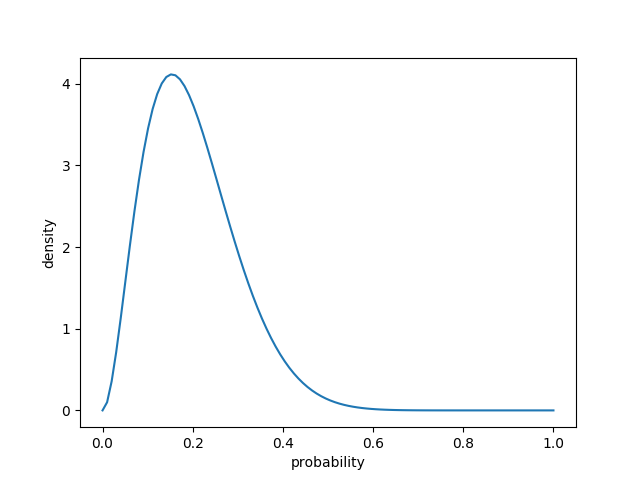
\includegraphics[scale=0.6]{distribution.png}
\caption{ density function of Beta-distribution}
\label{fig: label}
\end{figure}

\item[b)] Take a sample of 1000 random numbers and plot a histogram     
\begin{minted}[bgcolor=bg,linenos,fontsize=\small,autogobble]{python}
random_samples = stats.beta.rvs(alpha, beta, size=1000)
plt.hist(random_samples, density=True, alpha=0.5)
plt.savefig('./distribution_hist.png')
\end{minted}

\begin{figure}[H]
\centering  
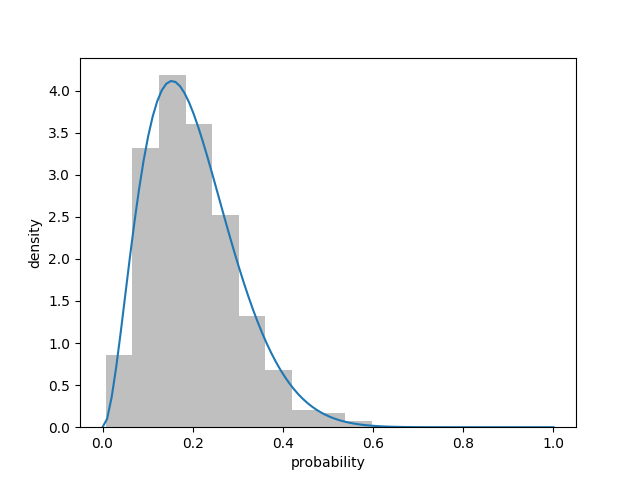
\includegraphics[scale=0.6]{distribution_hist.png}
\caption{histogram of 1000 samples}
\label{fig: label}
\end{figure}

\item[c)] Compute the sample mean and variance from the drawn sample

\begin{minted}[bgcolor=bg,linenos,fontsize=\small,autogobble]{python}   
sample_mean = np.mean(random_samples)
sample_variance = np.var(random_samples)
print('sample mean: ', sample_mean)
print('sample variance: ', sample_variance)
\end{minted} 

Sample mean:  0.19936416481824012\\
Sample variance:  0.009874950476577216

\item[d)]Estimate the central 95\%-interval of the distribution from the drawn samples
\begin{minted}[bgcolor=bg,linenos,fontsize=\small,autogobble]{python}   
sample_percentile = np.percentile(random_samples, q=2.5), 
                    np.percentile(random_samples, q=97.5)
print('sample central percentile 95%: ', sample_percentile)
\end{minted}      

Sample central percentile 95\%:  (0.04437716914185335, 0.4501785407399954)
\end{itemize}

\section{Bayes' theorem}

Given Event C: test subject has lung cancer, Event Y: test gives a positive result. \\

$P(C)=0.001,\ P(Y|C)=0.98,\ P(Y)=0.999\times0.04+0.001\times0.98=0.04094$, \\

According to Bayes' theorem, $P(C|Y)=\frac{P(Y|C)P(C)}{P(Y)}=0.02393$\\

We could see the probability of a random selected test subject having cancer given a positive result is 2.393\%. I would suggest researcher to improve their prediction accuracy and attach more importance to other factors causing cancer rather than test results ,e.g. families cancer history, bad habits, etc. These could reduce P(C).


\section{Bayes' theorem}

\begin{itemize}

    \item[a)] 
    $P(red)=0.4\times\frac{2}{7}+0.1\times\frac{4}{5}+0.5\times\frac{1}{4}=0.3193$\\
    
    The probability of picking a red ball  is 31.93\%.
    
    \item[b)] 
    $P(A|red)=\frac{P(red|A)P(A)}{P(red)}=0.3579$\\
    
    $P(B|red)=\frac{P(red|B)P(B)}{P(red)}=0.2505$\\
    
    $P(C|red)=\frac{P(red|C)P(C)}{P(red)}=0.3914$\\
    
    If a red ball was picked, it most probably came from box C.
    
\end{itemize}
\section{Bayes' theorem}

Given: Event $S$ is a notation of same gender twins, $I$ stands for identical twins and $F$ means fraternal twins. We need to find $P(I|S)$.\\

$P(S) = P(I) + P(F\ for\ the\ same\ gender) = \frac{1}{300} + 0.5 \times \frac{1}{125} = 0.0073$\\

$P(I|S) = \frac{P(Elvis\ being\ twin) \times P(I)}{P(S)} = \frac{1 \times\frac{1}{300}}{0.0073} = 0.45$\\

The probability that Elvis was an identical twin is 45\%.



\end{document}